\section{RQ3. Como os pacotes clientes se recuperam das \textit{breaking changes}?}

\subsubsection{A maioria das \textit{breaking changes} são introduzidas pelos provedores indiretos}

As \textit{breaking changes} também podem ser introduzidas pelos provedores indiretos e propagadas para os clientes. A Tabela \ref{tab:dependency_tree_deep} apresenta a profundidade/nível da árvore de dependência do cliente que o provedor que introduziu a \textit{breaking change} estava. Apenas 42.2\% das \textit{breaking changes} são introduzidas pelo provedor que o cliente realmente instalou e usa no seu código, ou seja, um provedor indireto que está referenciado no \textit{package.json} do cliente. Esses provedores estão no primeiro nível da árvore de dependências.

\begin{table}
	\centering
	\caption{O quão profundo o provedor que introduzia a \textit{breaking change} está do cliente na árvore de dependências}
	\begin{tabular}{lrr}
		\toprule
		\textbf{Nível} & (\#) & \textbf{\%} \\ \hline
		1              & 27   & 42.2\%       \\
		2              & 30   & 46.9\%       \\
		$>$3           & 07   & 10.9\%       \\ \bottomrule
	\end{tabular}
	\label{tab:dependency_tree_deep}
\end{table}

Um fato interessante é que as \textit{breaking changes} introduzidas pelos provedores indiretos, aqueles que estão no nível dois, três e quatro, representam 57.8\% dos casos. Seis casos estão no terceiro nível e um único caso está no quarto nível. Esses provedores não são instalados pelos clientes, mas eles são descarregados pelo \textsf{npm} quando o provedor direto é instalado. Nesses casos, a \textit{breaking change} podem ser totalmente desconhecida para os pacotes clientes, uma vez que os clientes podem não ter conhecimento sobre esses provedores.

\subsubsection{\textit{Breaking changes} que são corrigidas pelos provedores sendo clientes}

Um pacote provedor é aquele pacote que outros pacotes dependem dele. Entretanto, quando o provedor possui algum provedor, o primeiro provedor pode ser considerado como um cliente do segundo provedor. Por exemplo, na árvore de dependências como a seguinte \texttt{cliente}$\rightarrow$\texttt{prov1}$\rightarrow$\texttt{prov2} -- o \texttt{cliente} é o pacote cliente que teve seus testes executados neste trabalho -- o \texttt{cliente} tem como seu provedor o pacote \texttt{prov1}, e \texttt{prov1} tem o pacote \texttt{prov2} como seu provedor, que é um provedor indireto do pacote \texttt{cliente}. Então, quando a \textit{breaking change} é introduzida pelo \texttt{prov2} e se manifesta em \texttt{prov1}, o \texttt{prov1} pode ser considerado como um pacote cliente de \texttt{prov2} uma vez que na árvore de dependências o \texttt{prov2} é um provedor direto de \texttt{prov1}. A partir desta perspectiva, os próximos resultados são apresentados considerando o pacote cliente como aqueles que são clientes do pacote que introduziu a \textit{breaking changes} -- exceto nos casos classificados como \textit{Provedores incompatíveis} (Subseção \ref{sec:qp2:results}), porque ambos os provedores devem ser considerados como provedores de \texttt{cliente}.

Nesse contexto, a Tabela \ref{tab:package_fix} apresenta qual pacote corrigiu a cada caso de \textit{breaking change}. A maioria das \textit{breaking changes} foram consertados pelos pacotes provedores. Uma vez que são eles quem introduziram a \textit{breaking change}, teoricamente, esse era o comportamento esperado. Os pacotes clientes -- aqueles que tiveram seus testes executados neste trabalho -- recuperaram-se das \textit{breaking changes} em 20.3\% dos casos. Por último, os provedores que são considerados como clientes do provedor que realmente introduziu a \textit{breaking change}, recuperam-se das \textit{breaking changes} em 18.8\% dos casos. Isso é ótima observação para os pacotes clientes, pois os provedores como clientes corrigem as \textit{breaking changes} muitas vezes. Então, quando a \textit{breaking change} não é corrigida pelo provedor que a introduziu, outro provedor, que é o cliente do provedor que introduziu a \textit{breaking change}, pode consertar a \textit{breaking change} e corrigir o erro no pacote cliente.

\begin{table}
	\centering
	\caption{Pacotes que consertaram a \textit{breaking change}}
	\begin{tabular}{lrr}
		\toprule
		\textbf{Consertado por} & (\#) & \textbf{\%} \\ \hline
		Provedor              & 32   & 50\%        \\
		Cliente               & 13   & 20.3\%      \\
		Provedor como cliente & 12   & 18.8\%      \\
		Não consertado        & 07   & 10.9\%      \\ \bottomrule
	\end{tabular}
	\label{tab:package_fix}
\end{table}

Entretanto, considerando os cliente e os provedores como clientes, as \textit{breaking changes} são consertadas pelos clientes em 39.1\% dos casos. Esse valor indica que geralmente os clientes têm a tarefa de se recuperarem das \textit{breaking changes}.

\subsubsection{Provedores como clientes são os pacotes que mais rápido corrigem as \textit{breaking changes}}

Quando uma \textit{breaking change} é introduzida, ela deve ser corrigida pelo provedor que a introduziu, pelo provedor como cliente ou pelo pacote cliente. A Tabela \ref{tab:fix_day} apresenta o tempo que cada pacote gastou para consertar os casos de \textit{breaking changes}. Em geral, as \textit{breaking changes} são consertadas em 7 dias pelo provedor que as introduziram. Mesmo considerando esse curto período de tempo, um grande número de clientes diretos e indiretos podem ser afetados pelas \textit{breaking change} enquanto elas não são corrigidas.

\begin{table}
	\centering
	\caption{Mediana dos dias que cada pacote gastou para consertar os casos de \textit{breaking changes} e o tempo que os clientes e provedores como clientes gastam para realizar um \textit{upgrade}/\textit{downgrade} na versão dos provedores}
	\begin{tabular}{lrrrrrr} \toprule
		\textbf{Corrigido por} & \textbf{Dias} & \multicolumn{2}{c}{\textbf{Recuperado de}} & \phantom{ab} & \multicolumn{2}{c}{\textbf{Tempo para}}
		\\
		\cmidrule{3-4} \cmidrule{6-7}
		&    & implícito    & explicito    && \textit{downg}.       & \textit{upgr}.       \\ \midrule
		Provedor        & 06 & \textemdash & \textemdash && \textemdash  & \textemdash \\
		Cliente          & 34 & 34          & 82          && 18.5         & 78          \\
		Prov. como Cliente & 04 & 4           & \textemdash && 125.5        & 4           \\ \hline
		\textbf{Total}  & \textbf{07} & \textbf{10.5} & \textbf{82} && \textbf{18.5} & \textbf{10.5} \\
		\bottomrule
		\label{tab:fix_day}
	\end{tabular}
\end{table}

No geral, os pacotes que mais rápido corrigem as \textit{breaking changes} são os provedores como cliente. Na verdade, a uma \textit{breaking change} somente existe quando ela se manifesta nos pacotes clientes, portanto, os provedores como clientes são os primeiros pacotes a serem afetados pelas \textit{breaking changes} e são os que realmente precisam se recuperar. Considerando os provedores e os provedores como clientes, as \textit{breaking changes} são corrigidas em uma mediana de 5 dias pelos provedores, enquanto que os clientes gastam 34 dias para se recuperarem das \textit{breaking chnages}. Então, os pacotes que devem corrigir as \textit{breaking changes} são os provedores e os provedores como clientes, uma vez que os clientes demoram para se recuperarem e, de acordo com a Tabela \ref{tab:package_fix}, os provedores e os provedores como clientes são os que corrigem a maioria das \textit{breaking change} (78.8\%). Finalmente, as \textit{breaking changes} indiretas -- aquelas corrigidas pelos provedores como clientes -- são consertadas 1.5 vezes mais rápidas do que as \textit{breaking changes} diretas.

\subsubsection{Como os clientes se recuperam das \textit{breaking changes}}

A Tabela \ref{tab:version_change} apresenta os dados sobre as formas que os clientes se recuperam das \textit{breaking changes}. Em 48 casos os clientes alteraram a versão de seus provedores -- mesmo quando os provedores consertam as \textit{breaking changes}. Apesar de ser a maneira mais fácil de se recuperaram das \textit{breaking chnages}, na maioria dos casos (71.4\%), ao invés de realizarem um \textit{downgrade}, os pacotes clientes realizam um \textit{upgrade} na versão de seus provedores. A partir desse resultado, foi verificado todos os casos onde os clientes e os provedores como clientes consertaram a \textit{breaking change} apenas alterando a versão do provedor antes do provedor ter consertado a \textit{breaking change}. Foi observado que os clientes e provedores como clientes realizam um \textit{upgrade} em 12 (52.2\%) casos de 23. Ou seja, mais da metade dos casos do qual os clientes e os provedores como clientes consertaram a \textit{breaking change}, os pacotes provedores já tinham versões mais atuais mas esses clientes não estavam usando essas novas \textit{releases}.

\begin{table*}
	\centering
	\caption{Como os pacotes clientes alteram a versão dos provedores após uma \textit{breaking change}}
	\begin{tabular}{lcccccccccccc} \toprule
		\textbf{Pacote} & \textbf{Total} & \multicolumn{2}{c}{\textbf{\textit{Upgr.}}} & \phantom{ab} & \multicolumn{2}{c}{\textbf{\textit{Downg.}}} & \phantom{ab} & \multicolumn{2}{c}{\textbf{Trocado}} & \phantom{ab} & \multicolumn{2}{c}{\textbf{Removido}}
		\\ \cmidrule{3-4} \cmidrule{6-7} \cmidrule{9-10} \cmidrule{12-13}
		           &    & (\#) & (\%) && (\#) & (\%) && (\#) & (\%) && (\#) & (\%) \\ \midrule
		Cliente     & 28 & 20   & 71.4 && 06   & 21.4 && 01   & 3.6  &&  01  & 3.6  \\
		Prov. como Cliente & 20 & 09   & 45.0 && 10   & 50.0 && 01   & 5.0  && \textemdash & \textemdash \\ \bottomrule
		\label{tab:version_change}
	\end{tabular}
\end{table*}

O número de \textit{downgrades} nos provedores como clientes pode explicar o motivo que eles corrigem as \textit{breaking changes} mais rápido que outros pacotes. Uma vez que os provedores como clientes também são provedores, eles devem consertar as \textit{breaking changes} o mais rápido possível, assim evitando a propagação das \textit{breaking changes}. Portanto, realizar um \textit{downgrade} para uma \textit{release} estável do provedor, na metade dos casos, é a maneira mais comum de se recuperar das \textit{breaking changes}. Finalmente, em uma pequena proporção, os provedores são removidos ou trocados após a introdução das \textit{breaking changes}. Isso mostra o quão dependente os pacotes cliente podem ser dos seus provedores.

\subsubsection{Os clientes geralmente alteram a versão do provedor, mas para o mesmo \textit{range}}

Geralmente, os clientes alteram a versão de seus provedores. Isso garante que o \textsf{npm} não irá instalar as versões prévias do provedor que são aceitas pelo \textit{range}. Entretanto, quando uma \textit{breaking change} se manifesta, é praticamente mandatório atualizar a versão do provedor. A Figura \ref{fig:semver_both} apresenta quando os clientes (gráfico da esquerda) e os provedores como clientes (gráfico da direita) atualizam a versão dos seus provedores.

\begin {figure} [h!]
   \centering
   \mbox {
        \subfigure[Clientes]{\label{fig:bc_documentation_mocha} 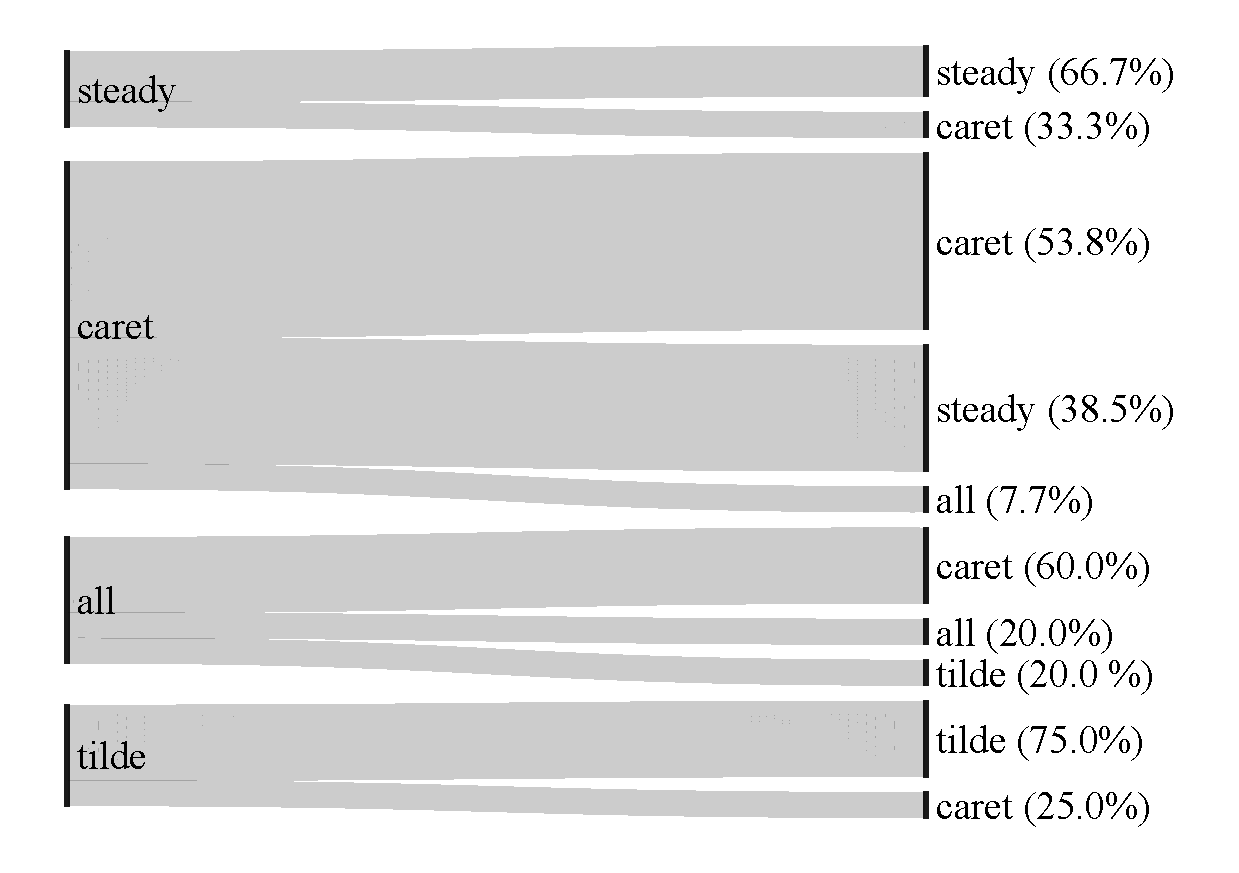
\includegraphics[scale=0.37]{figuras/semver_change_client.pdf}}\quad
        \subfigure[Provedores como clientes]{\label{fig:bc_documentation_other} 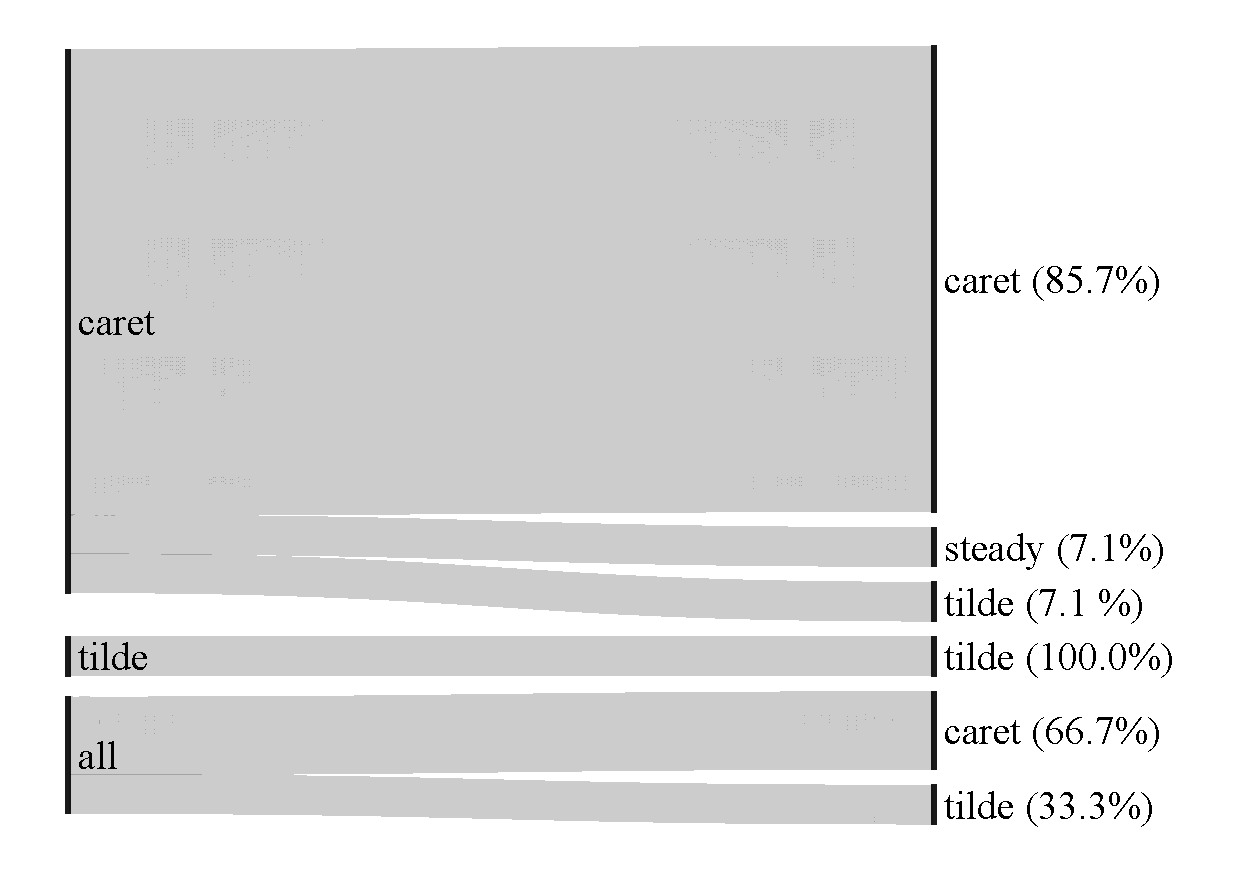
\includegraphics[scale=0.37]{figuras/semver_change_pac.pdf}}
    }
    \caption{A versão dos provedores alteradas pelos clientes e pelos provedores como clientes}
    \label{fig:semver_both}
\end{figure}

% \begin{figure}[]
%   \subfloat[Clientes]{
% 	\begin{minipage}[c][0.5\width]{0.5\textwidth}
% 	   \centering
% 	   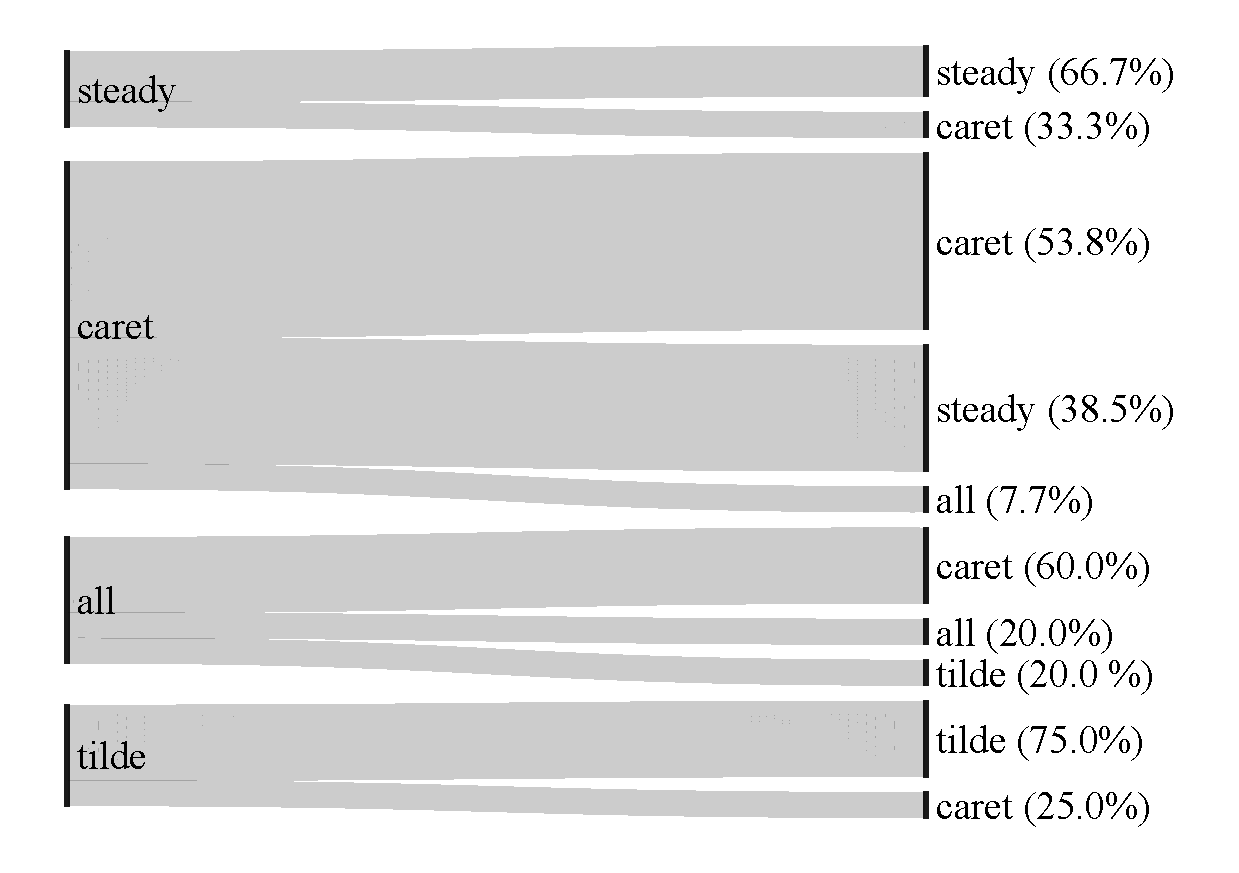
\includegraphics[width=0.7\textwidth]{figuras/semver_change_client.pdf}
% 	\end{minipage}}
%  \hfill
%   \subfloat[Provedores como Clientes]{
% 	\begin{minipage}[c][0.5\width]{0.5\textwidth}
% 	   \centering
% 	   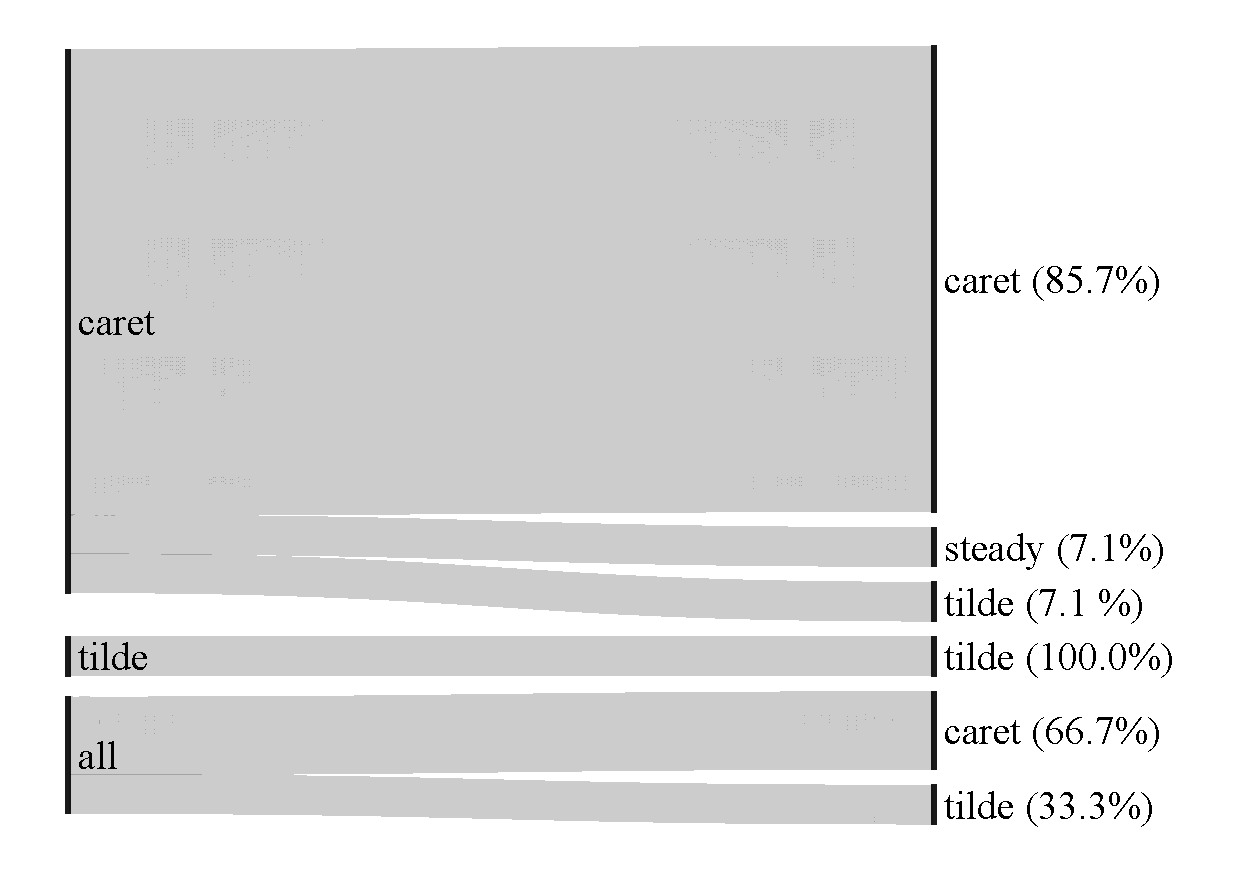
\includegraphics[width=0.7\textwidth]{figuras/semver_change_pac.pdf}
% 	\end{minipage}}
% \caption{A versão dos provedores alteradas pelos clientes e pelos provedores como clientes}
% \label{fig:semver_both}
% \end{figure}

Foi verificado que os provedores como clientes nunca utilizam a versão de seus provedores como \textit{steady}, ou seja, sem o \textit{range}. Quando uma \textit{breaking change} é manifestada nos provedores como clientes, eles sempre estão usando os seus provedores com um \textit{range}. Entretanto, apenas em um único caso o provedor como cliente alterou o \textit{range} de um \textit{caret} para um \textit{steady}. Mas, quando os clientes estão usando um \textit{range caret} e são impactados por uma \textit{breaking change}, em 38.5\% dos casos, eles realizam um \textit{downgrade} na versão do provedor alterando para um \textit{range steady}. Essa é a maneira mais rápida e fácil de se recuperar de uma \textit{breaking change}, mas o empecilho está no fato de se utilizar uma versão antiga do provedor.

A maioria das \textit{breaking changes} são introduzidas quando os clientes e provedores como clientes estão usando o \textit{range caret}. Esse é o \textit{range} padrão que o \textsf{npm} insere no \textit{package.json} quando um provedor é instalado. Mais da metade dos casos, esses clientes alteram a versão dos provedores para outro \textit{range caret}. Ainda, os \textit{X-range} são os menos usados e os apenas uma minoria de alteração de \textit{range} é convertida para um \textit{X-range}.

Os clientes e provedores como clientes tendem a manter o mesmo \textit{range}, apenas atualizando esse \textit{range}. Em 60.5\% dos casos, o tipo do \textit{range} (\textit{X-range}, \textit{range caret}, \textit{range tilde} ou \textit{steady}) é mantido, mas é realizado um \textit{downgrade/upgrade} no \textit{range} do provedor. Por exemplo, um cliente especifica o provedor como \textsf{p@\textasciicircum1.2.0} e recebe uma \textit{breaking change} em \textsf{p@1.3.2}, se o provedor corrige o erro, o cliente irá atualizar para, por exemplo, \textsf{p@\textasciicircum1.4.0}, mas não irá mudar para outro tipo de \textit{range}, tal como o \textit{range caret} ou o \textit{range tilde}.

\subsubsection{As \textit{breaking changes} documentadas são corrigidas 3.3 vezes mais rápidas do que as \textit{breaking changes} não documentadas}

Breaking changes podem ser documentadas em \textit{issues}, \textit{pull-requests} ou \textit{changelogs}. Tais documentações ocorrem em 78.1\% dos casos. A documentação afeta diretamente o tempo gasto para corrigir uma \textit{breaking change}. As \textit{breaking changes} que possuem pelo menos um tipo de documentação são corrigidas, em mediana, 3 dias após serem introduzidas. Em oposição, quando as \textit{breaking changes} não são documentadas elas recebem uma correção somente após 10 dias. Então, a documentação é muito importante para os clientes e os provedores quando eles estão tentando rastrear e corrigir as \textit{breaking changes}

\begin{mdframed}
Os pacotes clientes, incluindo os clientes diretos e os provedores como clientes, corrigem as \textit{breaking changes} em 39.1\% dos casos. Os casos de \textit{breaking changes} introduzidas pelos provedores indiretos são os mais comuns. Também, os provedores corrigem as \textit{breaking changes} mais rápidos do que os clientes, e os clientes preferem realizar um \textit{upgrade} a um \textit{downgrade} na versão do provedor. Finalmente, o \textit{range} dos provedores podem ser alterados após uma \textit{breaking changes}, mas, no geral, os clientes não alteram o tipo do \textit{range}. As \textit{breaking changes} documentadas são corrigidas 3.3 vezes mais rápido do que as demais.
\end{mdframed}